% Made up for the tikra benchmark.
% The flower of life: nineteen circles of the same radius, centered on a hexagonal lattice.
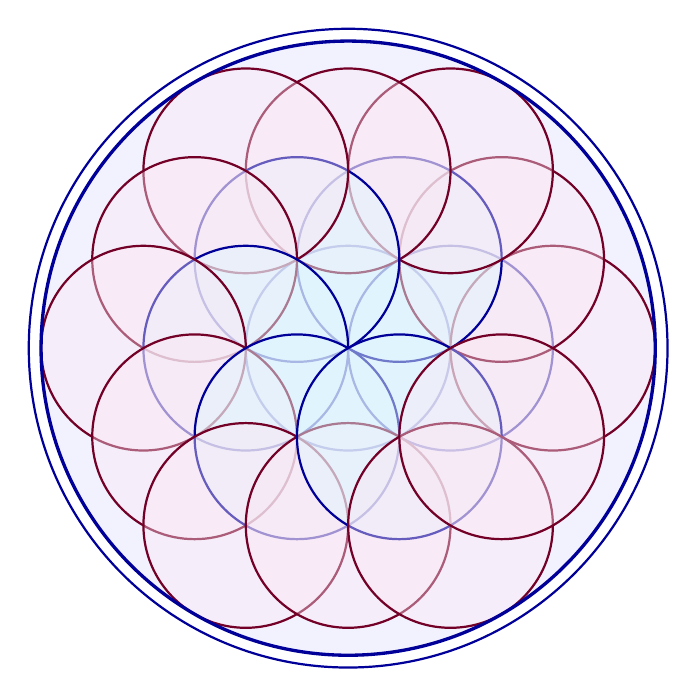
\begin{tikzpicture}[scale=1.3]
  \fill[blue!5] (0,0) circle (3);
  \foreach \r/\n in {0/1, 1/6, 2/12} {
    \ifnum\r=0
      \draw[blue!60!black, thick, fill=cyan!12, fill opacity=0.5] (0,0) circle (1);
    \fi
  }
  \foreach \a in {0,60,...,300} {
    \draw[blue!60!black, thick, fill=cyan!12, fill opacity=0.5] (\a:1) circle (1);
    \draw[purple!60!black, thick, fill=magenta!10, fill opacity=0.4] (\a:2) circle (1);
    \draw[purple!60!black, thick, fill=magenta!10, fill opacity=0.4] (\a+30:1.732) circle (1);
  }
  \draw[blue!60!black, very thick] (0,0) circle (3);
  \draw[blue!60!black, thick] (0,0) circle (3.12);
\end{tikzpicture}
